\documentclass[a4paper, 12pt]{article}
\usepackage{graphicx}
\usepackage{float}

\begin{document}

\section{Siemens IT Sec}
	\subsection{Secure Coding}
		\begin{itemize}
			\item Fehler und Verwundbarkeiten wärend des Betriebs auszubessern ist teuer.
			\item Ziel: Schwachstellen waehrend der Design- und Implementierunsphase zu erkennen und zu beheben.
		\end{itemize}
	\subsection{STRIDE}
	STRIDE Methode um Risk Scenarious und Worst-Cases festzulegen. Dabei werden folgende Aspekte behandelt:
	\begin{itemize}
		\item Spoofing Identity \\
		Das erlangen von Authentifizierung Informationen (Username und Password)
		\item Tampering with data \\
		Modifizieren von Daten um Schaden zu verursachen (schwierig zu erkennen, man muss alle Daten ueberpruefen wenn es irgendwann auffaellt).
		\item Repudiation \\
		Eine zulässige Transaktion wird von einem Teilnehmer (gefaelscht) nicht anerkannt.
		Non-Repudiation heißt im gegensatz dazu das alle Teilnehmer verfiziert werden koennen.
		\item Information disclosure \\
		Angreifer hat Zugriff auf sensitive Informationen.
		\item Denial of Service (DoS) \\
		Auslastung des Systems um berechtigte User daran zu hindern dieses zu benutzen.
		\item Escalation of privilege \\
		Ein Benutzer erhaelt/verschafft sich mehr Rechte als ihm zustehen.
	\end{itemize}
	\subsection{Security Assessment}
	Security Assessment beinhaltet pruefen und festlegen der Sicherheitsbeduerfnisse eines Assets (Geschaeftskritisches Objekt). \\
		\subsubsection{Assessment Process} 
		(siehe Foliensatz 1, Folie 42): \\
		Besteht aus mehreren Schritten, wird von versch. Dingen beeinflusst (Dokumentation, Vorschriften, Risiko Szenarien/Ziele, Attack patterns, ...)
		\begin{itemize}
			\item Technology and Threat Modeling Workshop: \\
			Workshop zum festlegen der Risiken, Vor-Ort mit Experten. Fuehrt zu einer detailierten Beurteilung der Assets.
			\item Security Assessment: \\
			59 Angriffsvektoren (zb. SQL Inj., Session Management), White-, Grey-, Blackbox, Auswirkung und Wahrscheinlichkeit. Diskussion ueber Architekturen, Coding Guidlines, Prozesse ...
			\item Reporting: \\
			Zusammenfassung fuer das Management, Gefundene Schwachstellen und Fehler, Praesentation und Uebergabe an den Kunden.
		\end{itemize}
	\subsection{Security Assurence Level (SAL)}
	Siemens teilt Angreifer in vier Level bezueglich ihrer Faehigkeiten ein.
	Umso hoeher der SAL desto mehr Aufwand ist noetig um sich zu schuetzen.
	\\\\
		\begin{tabular}{cccc}
			Angreifer & Methoden & Targeting & SAL \\
			Script Kiddy & Password Guessing, einfache Tools & non-targeted &  \\
			Opportunity Rider & URL veraendern, fortgeschr. Tools & surf-by & 1 \\
			Skilled Attacker & Injection, Professionelle Tools & semi-targeted & 2 \\
			Professional Attack & Logische und mehrstufige Angriff & targeted & 3 \\
			& Zugriff auf Source Code & & \\
		\end{tabular}

\section{WebSec}
\subsection{Black and Whitebox testing}
	\large Blackbox:
	Testumgebung bei der wenig bis keine Informationen über das System vorliegen.
	\large Whitebox:
	Testumgebung bei der genauere Informationen über das zu testende System vorliegen.
\subsection{OWASP Top 10}
	\large OWASP (Open Web Application Security Project)
	\large Goals:
	\begin{itemize}
		\item "identifying some of the most critical risks"
		\item "to raise awareness about application security"
		\item "not an application security program"
	\end{itemize}
	\large Top 10:
	\begin{enumerate}
		\item Injection
		\item XSS
		\item Broken Authentication and Session Management
		\item Insecure ddirect object references
		\item XS request forgery
		\item Security misconfiguration
		\item Insecure cryptographic storage
		\item Failure to restrict URL access
		\item Insufficient transport layer protection
		\item Invalidated redirects and forwards
	\end{enumerate}
\subsection{SQL Injection}
One of the most exploited vuln., despite being well known for almost a decade
\begin{itemize}
\item Problem: App doesn't properly separate database statements form user data
\item Impact: Read/Write access to database (sometimes even databases form other apps which are on the same server)
\item Tool support: sqlmap (can find injection, dump content, supports different DBMS)
\item Solution: Never trust user-supplied data - Separate query logic form user data
\item Good Practice: Prepared statements
\end{itemize}
\subsection{REST}
Representational State Transfer ist ein Programmierprinzip für Webanwendungen bei dem eine dynamsich generierte Seite den Inhalt einer serverseitigen Aktion darstellt. (Anzeigen von Suchergebnissen)
\large Eigenschaften die ein REST erfüllen muss:
\begin{itemize}
	\item Adressierbarkeit
	\item Underschiedliche Repräsentationen
	\item Zustandslosigkeit
	\item Operationen
	\item Verwenden von Hypermedia
\end{itemize}

\section{WebSec 2}
\subsection{SQL Injection}
$ //TODO sollte aehnlich zum punkt sql inj weiter unten sein $
\subsection{Other Injection}
Other interpreters to inject data e.g. OS shell, LDAP, XPath \\
\begin{itemize}
\item Example: OS commands often used for resizing images, copying files, start additional services
\item Injection: userdata gets part of OS command
\item Impact: depends on interpreter, most likely full system compromise
\item Solution: never trust user-supplied data. user data must be validated or escaped
\item Validation/Escaping: Whitelisting (RegEx), enclose in quotes, escape special characters
\item Tools: Burp Suite Scanner (commercial version only)
\end{itemize}

\subsection{XSS}
Attacker injects JavaScript code that get executed in the browser of web site visitors.\\

Problem:
\begin{itemize}
\item user data containing HTML markup is not properly escaped and included in the web server response
\item the browser renders the code of the attacker as part of the web page
\end{itemize}

\section{Security Challanges}
\subsection{Attackermodel}
Wikipedia: Attack models or attack types specify how much information a cryptanalyst has access to when breaking or cracking an encrypted message, commonly known as codebreaking or cracking the code. 
\large Some common attack models are:
\begin{itemize}
	\item Ciphertext-only attack
	\item Known-plaintext attack
	\item Chosen-plaintext attack
	\item Chosen-ciphertext attack
\end{itemize}
\subsection{Standartmodel}
ACHTUNG - Meine Interpretation aus den Folien, die btw scheiße sind.
Standard model heißt das der Intruder den Nachrichten verkehr von Alice und Bob mithört und entschlüsselt. (Bsp. Man in the Middle)
Non-Standard model heißt der Intruder hört nicht die Nachrichten von Alice und Bob ab sonder manipuliert ihre Endgeräte oder sie selbst und holt sich die Inforamtionen noch bevor sie auf den weg geschickt werden. (Troja-Horse, Social attacks)
\subsection{Dolev-Yao}
Ein Model um die Sicherheit von Protokollen zu beweisen. Annahmen über die kryptologischen Bestandteile des Protokolls, den Angreifer, das Netzwerk sowie dessen Teilnehmer helfen beim treffen von formalen Aussagen.
\subsection{Needham-Schroeder-Protokoll}
Ein Protokoll für sicheren Datenaustausch in einem dezentralen Netzwerk, das den Schlüsselaustausch und die Authentifikation mit einem Ziel vereint.
\large Ablauf:
\begin{enumerate}
	\item Alice schickt eine mit dem public key KeyB verschlüsselte Nachricht die ein shared secret nA und die Identität von Alice A enthält an Bob.
	\item Bob entschlüsselt die Nachricht mit seinem private key und antwortet Alice mit einer verschlüsselten Nachricht die das shared secret von Alice nA und ein shared secret von Bob nB enthält. Die Nachricht wird mit dem public key von Alice KeyA verschlüsselt.
	\item Alice entschlüsselt die Nachricht mit ihrem private key und sendet Bob eine verschlüsselte Nachricht die das shared secret von Bob nB enthält. Die Nachricht wird mit dem public key von Bob KeyB verschlüsselt.
\end{enumerate}
\begin{figure}[H]
\centering
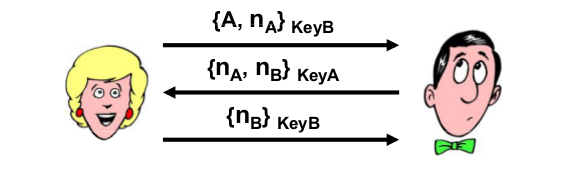
\includegraphics{./img/ns_01}
\label{fig:ns_01}
\end{figure}
\large Problem bei dieser Methode ist:
Bringt der Intruder Alice dazu eine Verbindung zu ihm aufzubauen, schickt Alice erst ihr shared secret an den Intruder. Dieser leitet die Nachricht an Bob weiter welcher mit seinem shared secret und dem von Alice antwortet. Hier kann der Intruder das shared secret von Bob noch nicht auslesen da die Nachricht mit dem public key von Alice verschlüsselt wurde, daher leitet der Intruder die Nachricht an Alice weiter. Alice antwortet DEM INTRUDER mit dem shared secret von Bob.
\newline
Der Intruder kennt nun das shared secret von Alice und Bob.
\begin{figure}[H]
\centering
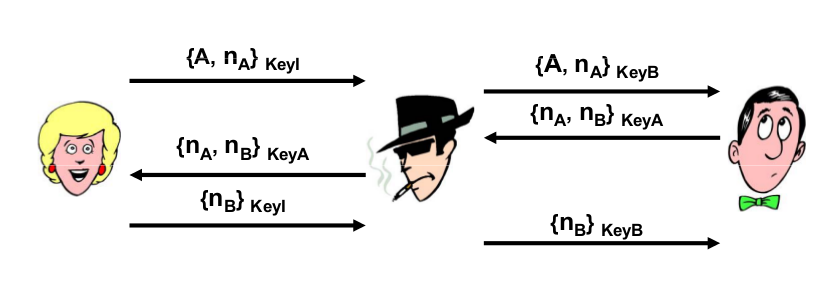
\includegraphics[width=\linewidth]{./img/ns_02}
\label{fig:ns_02}
\end{figure}
\large Lösung:
Bob schickt seine Identität mit. (Bin mir nimma ganz sicher sollten wir am So nochmal bereden :D)

\subsection{Models for the Attacker}
\begin{itemize}
	\item Man-in-the-middle attack
	\item Trojan Horses
	\item Read Hard Disk on another system
	\item Read data in Smart Cards via side-channels(e.g. Energieverbrauch)
	\item Social attacks (Social engineering)
	\item Shoulder surfing (Camera on your office)
\end{itemize}
\subsection{Three meanings of "For all x there is a y"}
	x = (Programm P, Input i) \newline
	y = 1 if P terminates with Input i, 0 if not
\begin{enumerate}
	\item Mathematical Meaning
	\item Constructive Meaning
	\item Complexity-dependent meaning(s)
\end{enumerate}
\subsection{Muenzwurf}
Odd numbers can be given by 4n+1 (Type +1) and 4n-1 (Type -1).\\
Fact:
\begin{itemize}
\item Multiplying two (odd) integers of the same type yield a product of Type +1.
\item Factoring a product of two large primes is not tractable.
\end{itemize}
Example:
\begin{itemize}
\item (4p+1)(4q+1) = 16pq+4p+4q+1 = 4(4pq+p+q)+1
\item (4p-1)(4q-1) = 16pq-4p-4q+1 = 4(4pq-p-q)+1
\end{itemize}
\begin{enumerate}
\item Alice randomly picks one of the two types b (flips coin). She multiplies two randomly chosen large primes P,Q of type b and sends the result N=PQ to Bob.\\
\item Bob guesses the type b' of the factors.\\
\item Alice reveals the prime factors so Bob can verify weather he has guessed b' correctly or not.
\end{enumerate}

\subsection{Dataflow}
Data Flow is the usually intended flow of data between parts of the system using explicitly defined channels. DataFlows crossing Trust Boundaries (domains) must be secured.//
Dataflow problems:
\begin{itemize}
\item sometimes unintended
\item sometimes a security risk, eg:
\begin{itemize}
\item standard interface exposes a file that should not expose
\item detailed error messages (file names or file locations -> directory traversal attack)
\end{itemize} 
\end{itemize}

Inadvertent Information Flow (Leakage):\\
\begin{itemize}
\item unvoluntary/unexpected pass of information
\item usually over a covert channel (timing, energy consumption, cache behaviour etc)
\item leaked information can be deduced from other legitimitely sent informations
\end{itemize}
\subsection{Security policies}
Eine security policy ist eine Liste von Zuständen die als secure oder authorized states bezeichnet werden. Alle zustände außerhalb werden als unauthorized bzw non-secure states bezeichnet. Policies werden durch so genannte security mechanisms umgesetzt.
\subsection{Non-Modularity}
Zwei unabhängige Systeme die einzeln als sicher gelten, müssen wenn man sie kombiniert nicht zwangsweise sicher sein.
\section{SmartGrid}
\subsection{Motivation}
\begin{itemize}
\item 70\% of urban population will live in cities by 2050
\item current energy supply afffected by:
\begin{itemize}
\item blackouts
\item power overloads
\item high costs
\end{itemize}
\item upcomming challenges
\begin{itemize}
\item distributed power supply
\item scarcity of resources
\end{itemize}
\end{itemize}
\subsection{Properties of SmartGrid}
\begin{itemize}
\item self-monitoring
\item auto-balancing
\item self-regulating
\item efficient
\item cost reducing
\end{itemize}

\subsection{Entities (Roles)}
\begin{itemize}
\item Energy Generators
\item Energy Suppliers
\begin{itemize}
\item data communication network
\item network gateway
\item energy supply server
\end{itemize}
\item Prosumer \& Home Domain
\begin{itemize}
\item Smart Appliances
\item Smart Meter
\item (Wireless) Home Area Network
\item Home Gateway
\item Home Energy Management System
\end{itemize}
\item Meter Point Operator
\end{itemize}


\subsection{Szenario}
\begin{figure}[H]
\centering
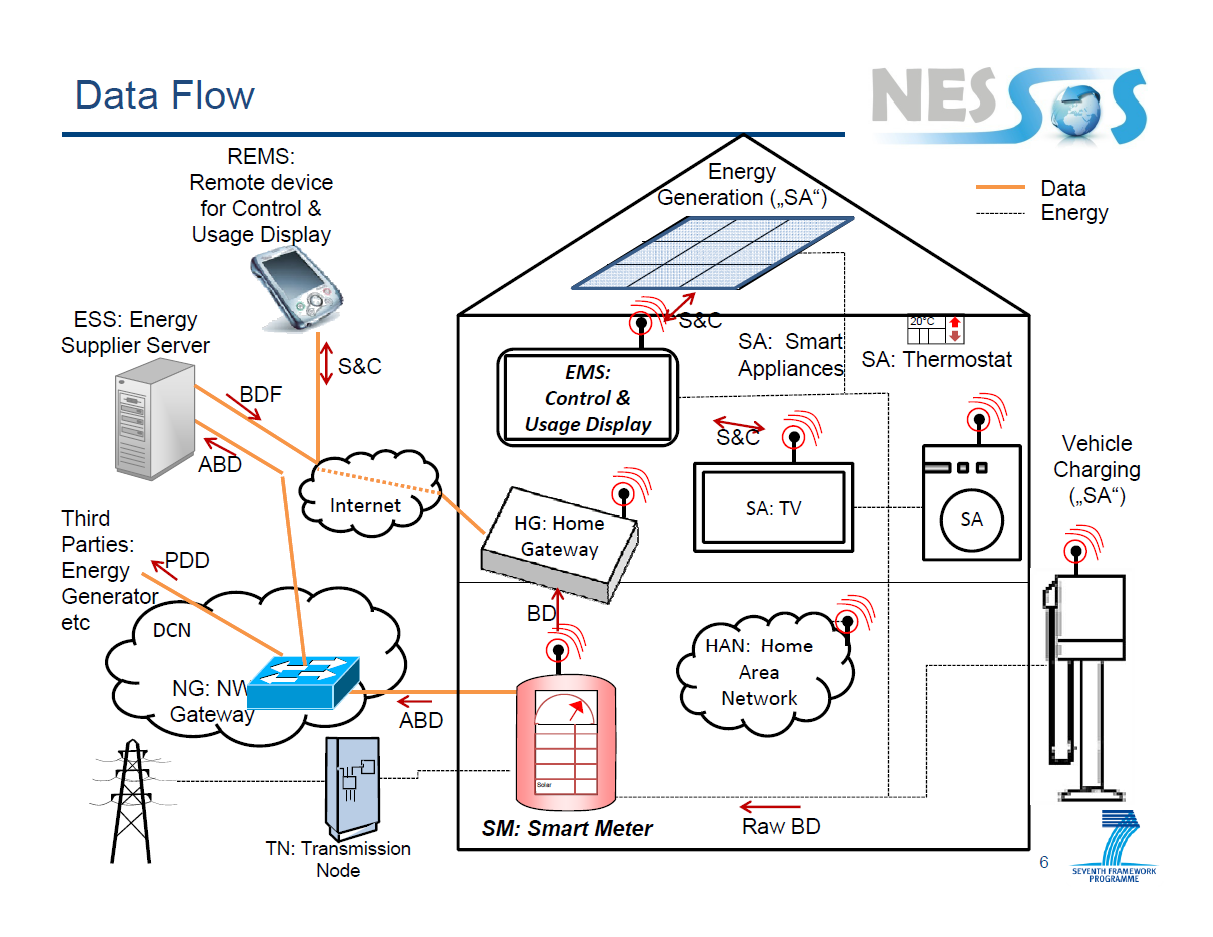
\includegraphics{./img/smartgrid_datablow}
\label{fig:smartgrid_datablow}
\end{figure}

\subsection{Which Attacks are Posible}
\subsubsection{Family with children}
\begin{itemize}
\item Which information could the attacker obtain?
\begin{itemize}
\item How many persons live?
\end{itemize}
\item Possible Tracking?
\begin{itemize}
\item Combination of informations useful for burglary etc
\end{itemize}
\end{itemize}

\subsubsection{Smart Appliances}
\begin{itemize}
\item Which appliances are "smart"?
\item What kind of information (R/S\&C) do the process?
\item What are the appliances' functionalities?
\item Can a successful attack to an appliance lead to a compromise of the AIM?
\end{itemize}

\subsubsection{Privacy}
\begin{itemize}
\item Initial assumption: all communication is encrypted
\begin{itemize}
\item Possible to read / disclose / etc information regardless of encryption?
\item Time / Communication / Parties / Message length etc, help disclose the payload data?
\item Possible to misuse insider status ( Prosumer / Energy Supplier)?
\end{itemize}
\end{itemize}

\subsubsection{Impersonation}
\begin{itemize}
\item How to impersonate another customer for accounting fraud?
\item Possible to impersonate a server?
\begin{itemize}
\item With which results?
\end{itemize}
\end{itemize}

\subsubsection{Encryption and Key Management}
\begin{itemize}
\item Assume: Communication is encrypted
\begin{itemize}
\item bypass the communication encryption?
\item extract keys or to intercept key exchanges or key updates?
\item exploit implementation weaknesses at the network/transport layer
\item exploit insider status?
\end{itemize}
\end{itemize}

\subsubsection{Electric Mobility}
\begin{itemize}
\item Assumption: Electric vehicles share an unique vehicle ID
\begin{itemize}
\item impersonation?
\item fraud?
\item tracing?
\item theft?
\end{itemize}
\end{itemize}

\subsection{Abrechnung und Steuerung im Privathaus}
\begin{itemize}

\item Raw Billing Data (RawBD)
\begin{itemize}
\item all related data, gathered by SmartMeter (SM)
\end{itemize}

\item Billing Data (BD)
\begin{itemize}
\item processed and stored by SM and local Energy Management System (EMS)
\end{itemize}

\item Aggregated Billing Data (ABD)
\begin{itemize}
\item Sent to the Network Gateway (NG) and forwarded to the energy supplier (ES)
\end{itemize}

\item Data for Power generation and Distributed Purpose (PDD)
\begin{itemize}
\item aggregated by ES from ABD of several houshold
\item usage forecasts for certain sectors
\end{itemize}

\item Billing Data Feedback (BDF)
\begin{itemize}
\item every ~5 minutes users are informed about usage, generation, costs, revenues and current rates
\end{itemize}

\item Status and Control (S\&C)
\begin{itemize}
\item local logon to the EMS
\item view and control Smart Appliances and Energy Management Policies
\end{itemize}

\item Remote Status and Control (RS\&C)
\begin{itemize}
\item see S\&C
\item using e.g. cellular phone or remote PC from external hot spots
\end{itemize}

\end{itemize}
\section{Internet of Things}
\subsection{Applikationbeispiele}
\begin{itemize}
	\item Electronic Notes on real locations \\
	Visitors can use a hand-held to place a note at any location in the real world.
	Other Visitors can add their own messages to it.
	Users can trigger actions on certain conditions.
	\item Information on products or advertisement \\
	Wireless devices can read autonomously information on products and feed them to the user.
	\item Traceability and counterfeiting support \\
	Instead of of barcodes, IoT is used to track products.
	Tackle counterfeiting, Tracking unsafe products.
	\item Sensors in Health Care \\
	Large amount of applications in mobile health. Example: Patient Monitoring
	\item Subervision, Command and Control Systems (plants, industrial facilities)
	\item Intelligent just-in-time manufacturing \\
	IoT-enabled materials, goods in production , machines and transport vehicles.
	The all parts of the system can communicate with each other.
	The system is aware of the production steps and can decide alone where the resources should be used. (Just-in-time supply of materials, autonomous reconfiguration and adaptation)
	\item Smart Grids \\
	Network of smart objects, designed to control a system in real time. Example: Home energy management to monitor and manage power consumption of running devices.
	\item Smart Cities \\
	Network of smart objects to manage traffic.
	Environmental monitoring to check on pollution, temperature, smoke, ...
	In and outside the city/buildings.
	\item Location-based services (LBS)
	Devices know their location (GPS). Leads to a large amount of applications.
	Examples:\\
	Today: \\
	Order a taxi, navigation systems, mobile advertising, proximity-based access control\\
	Future: \\
	Rescue troops detect people in danger, smart homes know which environment to use depending on the user, manufacturing (see Intelligent just-in-time manufacturing).
\end{itemize}
\subsection{Sec Challanges}
$ //TODO combine the following points better // nicht gar so wichtig sind aber par sachen doppelt vom inhalt her$
\begin{itemize}
\item larger attack surface
\begin{itemize}
\item large number of interfaces
\item new possibilities of exploiting existing vuln. and threats
\item new interaction possibilities
\item new possible attack patterns or procedures, threats and damages
\item IoT devices use local and remote services and provide services with or without any human intervertion
\end{itemize}
\item Fault Tolerance
\begin{itemize}
\item Connectivity is not constant
\item context of devices changes over timem sometimes abruptly
\item system must cope with these changes, providing a partial service until the conditions are more facorable
\end{itemize}
\item Efficient Cryptographic Primitces
\begin{itemize}
\item provide good secirity primitives suitable for low resource consumption(energy, time, sace)
\item deployment of efficient key distribution and management systems
\end{itemize}
\item Integrate IoT with the rest of the Internet
\begin{itemize}
\item use protocols and security mechanisms used in the internet or bridge to them, archieving end-to-end security when translating the different underlying protocols, existence of such sub-networks and interactions between them must be taken into account
\end{itemize}
\item Intrusion Detection Systems and Survivability Mechanisms
\begin{itemize}
\item react to changes in environment
\end{itemize}
\item Trust Management and Secure Collaboration
\begin{itemize}
\item Need trust relationships between users and devices
\item Devices might know each other, or might be complete stranges
\item Need to interoperate the security policies of different components(how will devices react if a particular event arises?, Who are the elements i should collaborate with, and how?)
\end{itemize}
\item Models and mechanisms for device and data ownership
\begin{itemize}
\item Users may utilize their devices to authenticate themselves
\item Devices might perform certain operations on behalf of their users
\item MEchanisms and security policies and mechanisms that control how the data is created, accessed and protected
\end{itemize}
\item Software maintenance process
\begin{itemize}
\item How to release security patches
\end{itemize}
\item Usability
\begin{itemize}
\item security for IoT-based applications must be understandable and manageable by end-users
\end{itemize}
\item Privacy
\begin{itemize}
\item "Things" belong to people and collect information about actions of them
\item Devices and interfaces should do not leak personal information aboit the users location activities preferences // haha nice try NSA :D
\item Need to avoid that a communication partner is able to collect large amounts of information. Current Algorithms do not prevent this type of attack
\end{itemize}
\end{itemize}

\subsection{Sec Solutions}
\begin{itemize}
\item Fast and secure network bootstrapping
\begin{itemize}
\item minimizing security attacks when network is initialized
\item objects don't have knowledge regarding environment and their neighbouring nodes
\end{itemize}
\item Secure and Context-aware dynamic auto configuration
\begin{itemize}
\item When a new Object enters its security settings and its config will be automatically distributed via the network
\end{itemize}
\item Self-management and self-monitoring mechanisms
\begin{itemize}
\item ensuring smooth operations and continuous monitoring to track problems
\item trigger self-healing algorithms for fault avoidance
\end{itemize}
\item Creation of a Run-time Security Reconfigurability Platform
\begin{itemize}
\item allowing the end-users app or service to request particular security servies or settings
\end{itemize}
\end{itemize}

\subsection{RFID}
\begin{itemize}
\item Passive Tags - no power source
\item small amount of data
\item RFID reader powers tag, extracts data via radion
\end{itemize}
\large Applications
\begin{itemize}
\item Authentication Authorization Access Control
\begin{itemize}
\item Patient and practitioner Identification Hospital
\item Car Keys
\item Passports
\item Secure Entry cards
\item Libary books
\end{itemize}
\item Supply chain managment (inventory control)
\item Payment systems
\begin{itemize}
\item I-Pass
\item Credit Card
\end{itemize}
\item Animal Tracking - and Human 
\begin{itemize}
\item VeriChip: Human implantable RFID tag, can penetrate mud, blood ,water, only the size of a rice grain
\item Emergency access to patient-supplied health information
\item Portable medical records access
\item Disease/treatment management of at-risk population
\end{itemize}
\end{itemize}
\large Conderns:
\begin{itemize}
\item Problem: "unintended consequences"
\item Read tags through briefcases, etc
\item Exp: Tracking books. Can we figure out what you're reading, and where you are?
\end{itemize}
\large Privacy Threats
\begin{itemize}
\item Tracking: Determine where individuals are or where they have been
\item Hotlisting: Single out certain individuals because of the items they possess
\item Profiling: Identifying the items an idividual has in their possession
\end{itemize}
A sufficiently powerful directerd reader reads tags in a house or car, enabling large scale tracking and profiling of individuals \\ \newline
\large Design Principles for Privacy
\begin{itemize}
\item Proportionality
\begin{itemize}
\item a balanced analysis of whether the risk to individuals is sufficiently mitigated to justify the use of RFID
\end{itemize}
\item Transparency
\begin{itemize}
\item ensure RFID is not secretly used to collect data (limited to a very close read range and crypto protection)
\end{itemize}
\item Notice
\begin{itemize}
\item individuals in RFID enabled environments should receive notification that the tech. is used, type of data collection, and how the data will be shared and used
\end{itemize}
\item Choice
\begin{itemize}
\item User has choice to disable tag at some point(if the tag is in an item the individual will carry with them)
\item disabling with zb. a blocker bag
\end{itemize}
\end{itemize}


\subsection{Baumbasierendes Model}
fuer RFID
$ //TODO $


\section{6 Threads Landscape}
\subsection{Phishing}
Fraudulent e-mails and legitimate looking websites by cybercriminals in order to deceitfully gain user credentials.
\subsection{Spearphising}
Phishing attempts directed at specific individuals or companies have been termed spearphishing. Attackers may gather personal information about their target to increase their probability of success. [Wikipedia]
\subsection{Rouge certificates}
Rogue certificates allow attackers to create illegitimate sites that are indistinguishable from real sites like eBay, Google or PNC because their certificate hierarchy can be validated.  Users then will be redirected to such sites through phishing or ‘”man in the middle” attacks where a compromised host in-between the user and a legitimate site sends traffic to an illegitimate site instead.
[Soße: http://www.jurinnov.com/the-threat-of-rogue-certificate-authorities]
Stuxnet, Duqu and Flamer used rouge certificates.
\subsection{Chain of Trust}
The Certificate Hierarchy is a structure of certificates that allows individuals to verify the validity of a certificate's issuer. Certificates are issued and signed by certificates that reside higher in the certificate hierarchy, so the validity and trustworthiness of a given certificate is determined by the corresponding validity of the certificate that signed it.
[Wikipedia]
\section{Cause Analysis}
\subsection{Implementation errors exploited via legitimate port}
Typical scenario would be specially crafted packets causeing buffer overflows to place codes or commands. (e.g. remote code executun, privilege escalation , data stealing, full control)

\section{Product certification and
formal security analysis
at industrial examples}
\subsection{Common Criteria}
	\subsubsection{Common Criteria process overview}
	Certification according to the Common Criteria is a rather complex, time
	consuming and expensive process, providing systematic assurance.
	A successful, approved evaluation is awarded a certificate.
	Lifetime of certificates is theoretically not bounded, but their
	applicability is limited by technical progress (re-certification).
		\begin{figure}[H]
		\centering
		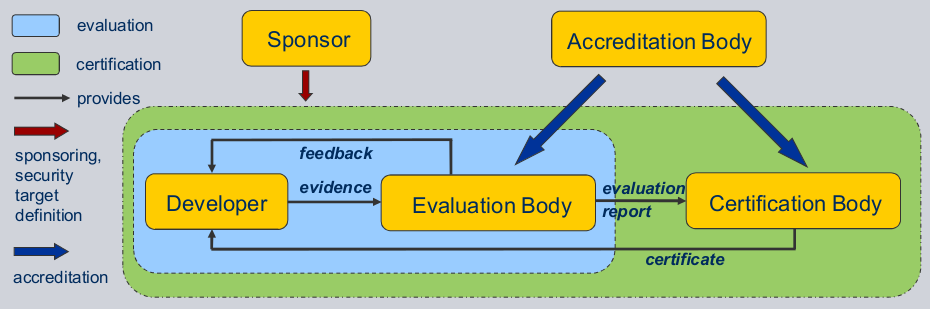
\includegraphics[width=1\linewidth]{./img/cc_01}
		\label{fig:cc_01}
		\end{figure}
	\subsection{Security requirements documents}
		Security Target (ST):
		defines extent and depth of the evaluation
		for a specific product called Target of Evaluation (TOE) \\
		Protection Profile (PP):
		defines extent and depth of the evaluation
		for a whole class of products, i.e. firewalls
	\subsubsection{Security Functional Requirements (SFRs) overview}
		\begin{itemize}
			\item	FAU: Security audit
			\begin{itemize}
				\item Security audit automatic response (FAU\_ARP)
				\item Security audit data generation (FAU\_GEN)
				\item Security audit analysis (FAU\_SAA)
				\item Security audit review (FAU\_SAR)
				\item Security audit event selection (FAU\_SEL)
				\item Security audit event storage (FAU\_STG)
			\end{itemize}
			\item	FCO: Communication
			\item	FCS: Cryptographic support
			\item	FDP: User data protection
			\item	FIA : Identification and authentication
			\item	FMT: Security management
			\item	FPR: Privacy
			\item	FPT: Protection of the TSF
			\item	FRU: Resource utilization
			\item	FTA: TOE access
			\item	FTP: Trusted path/channels
		\end{itemize}
	\subsubsection{Evaluation Assurance Levels}
		\begin{tabular}{|c|c|} \hline
		\textbf{} & \textbf{ELA designation} \\ \hline
			EAL1 & functionally tested \\ \hline
			EAL2 & structurally tested \\ \hline
			EAL3 & methodically tested and checked \\ \hline
			EAL4 & methodically designed, tested and reviewed \\ \hline
			EAL5 & semiformally designed and tested \\ \hline
			EAL6 & semiformally verified design and tested \\ \hline
			EAL7 & formally verified design and tested \\ \hline
		\end{tabular} \\ \\
		EAL does not say how secure a product is, but how well its requirements are checked.
		Assurance is grounds for confidence that an IT product meets its security objectives.
		\subsection{Factors determining the evaluation effort}
			\begin{itemize}
				\item Boundary of TOE vs. TOE environment
				\item Definition of Threats and Security Objectives for the TOE
				\item Definition of Security Functional Requirements (SFRs)
				\item Selection of Evaluation Assurance Level (EAL)
			\end{itemize}
\subsection{Was ist ein Sec Target}
$ //TODO $
\subsection{Was ist ein Connection Profile}
$ //TODO $
\subsection{Security function requ}
$ //TODO $
\subsection{Security assurance requ}
$ //TODO $
\subsection{Was sind EALs}
$ //TODO $

\section{Web Vulnerabilities}
\subsection{State-of-the-art security measures}
\begin{itemize}
	\item Application	
	\begin{itemize}
		\item High password quality
		\item User input validation
		\item Lock-out mechanisms (5 login failues, ...)
	\end{itemize}
	\item Firewall
	\begin{itemize}
		\item Encrypted tunnel - only https://
		\item Restrictive Firewall policy - only secure traffic permitted
	\end{itemize}
	\item Server
	\begin{itemize}
		\item Server Hardening - Only really needed software is running on the server, users only have limited privileges, ...
		\item Intrusion detection systems (ex. snort)
		\item Lates patches installed
		\item Anti-virus
	\end{itemize}
\end{itemize}

\subsection{Top 10}
Siehe OWASP oben 2.2, hier eine weiter nicht offizielle OWASP Top10 (weder 2010, noch 2013). Empfehle dieses OWASP zu ignorieren.
\begin{itemize}
\item XSS
\item Injection Flaws
\item Malicious File Execution
\item Insecure direct object reference
\item CSRF
\item Information Leakage and Improper Error Handling
\item Broken authentication and session management
\item Insecure Cryptographic Storage
\item Insecure Communications
\item Failure to restrict URL access
\end{itemize}
\subsection{SQL Injection}
Typical Code: \\
string sql = "select * from Users where user ='" +
User.Form + "' and pwd='" + Password.Form + "'"\\\\
Attacker: \\
sql="select * from Users where user ='mch160' and pwd
='' or 1=1 -- '"\\\\

Some commands:
\begin{itemize}
\item 'or 1=1 --'   = login without password
\item '; drop database myDB; --   = delete database
\item '; xp\_cmdshell 'format c: /q /yes   = format harddrive (MSSQL Server)
\end{itemize}
Database system usually runs with system privileges ...

\subsubsection{Counter Measures}
\begin{itemize}
\item Limit user access
\item Limit user input length and data types
\item Verify data types
\item Quoting the input and filter out characters (\textbackslash, /, ;, --, ...)
\item Proper error handling
\item Prepared statement or parameterized statement \\
\begin{itemize}
\item // 1. define statement (query logic): \\
PreparedStatement ps = Connection.prepareStatement(
"SELECT user, password FROM tbl\_user WHERE (user=?)"
);
\item //2. bind query parameters to user input \\
ps.setString(1, username);
\item //3. execute query \\
ResultSet rs = ps.executeQuery();
\end{itemize}
\item Stored Procedures \\
Procedures are stored in the Database and called with the give input parameters.
Disable stored procedures master (XP\_cmdshell, XP\_startmail,...)
\end{itemize}

\subsection{XSS - Cross-site scripting}
\begin{itemize}
\item User injects JavaScript code that subsequentially gets executed in the browser of the visitor
\item Problem: User data that contains HTML markup is not properly escaped, the browser renders the attacker code as part of the web page
\end{itemize}

\subsection{CSRF}
\subsection{Session Hacking}
//Broken Authentication and session mgmt.
\begin{itemize}
\item Badly implemented access control: index.html redirects to secret.html if the password is correct
\item Sometimes one can go directly to secret.html without password check
\end{itemize}

\section{Formal Security Models}
\subsection{Welche art von Modellen gibt es}
$ //TODO $
\subsection{Ansatz und Vorteile von Formal Security}
$ //TODO $
\subsection{Conclusions}
$ //TODO $

\section{BufferOverflow}
\subsection{Buffer Overflows}
Things good to know:
\begin{itemize}
\item First publication 1972
\item First documented exploit, Morris Worm 1988
\item Three famous Worms(2001 Code Red Worm, 2003 SQL Slammer, 2008 Conficker Worm)
\item Triggered by external data input with Dangerous code
\item Mostly seen in C/C++ because of missing memory boundarys or access checking
\end{itemize}
\subsubsection{Stack Buffer Overflows}
Programm Stack: used for managing prog execution and prog state, saves 
\begin{itemize}
\item Return Address
\item Function Arguments
\item Local Varibales
\end{itemize}
on the Stack Frame.
Register EBP saves actual address of the Frame (Intel)
Frame Pointer is the Reference Pointer within the Stack
Stack gets modified during following actions
\begin{itemize}
\item Function call
\item Function Initialization
\item When function returns
\end{itemize}
$ //TODO merge FunctionCall example $
\subsubsection{Heap Buffer Overflows}
Ich denke hierzu haben wir nicht wirklich was gemacht weis nicht ob das jedoch bekannt ist

\subsection{Basic Errors}
\begin{itemize}
\item Strings
\begin{itemize}
\item Unbounded String Copies
\item Off-by-One Errors
\item Null-Termination Errors
\item String Truncation
\end{itemize}
\item Memory Managment Errors
\begin{itemize}
\item Double Free
\end{itemize}
\item Integer
\begin{itemize}
\item Integer Overflow
\item Sogn Errors
\item Truncation Errors
\end{itemize}
\item Formated Output
\begin{itemize}
\item Format String
\end{itemize}
\end{itemize} 

\subsection{Code Injection}
\begin{itemize}
\item Attacker creats malicious argument
\item The argument is a string which includes a pointer to the malicious code
\item When the function return, the maliciouse code is executed
\item The malicious code has the same permissions as the program exploited
\end{itemize}
\large Malicious Argument
\begin{itemize}
\item Program must interpret the input as legitimate input
\item The argument must allow the attacker to execute his code
\item The argument should not crash the attacked program
\end{itemize}
\large Malicious Code
\begin{itemize}
\item Code can be part of the argument but mostly is injected through a different vector
\item Code has the ability to execute every functionality which can be programmed; mostly remote shell on targeted system
\end{itemize}

\subsection{Return to libc}
\begin{itemize}
\item In the Return to libc the attacker modifies the Return Address to point to a function which is already in the address space(libc)
\item This allows to inject new functionality to be executed during the normal application execution.
\item Injecting addresses of existing functions e.g. system() exec()
\end{itemize}
Exploit
\begin{enumerate}
\item Overwrite the return addresse with an address of a existing libc function
\item Create a Stack Frame to execute other functions
\item Restore the original Stack Frame to execute the original application
\end{enumerate}
Interesting, because:
\begin{itemize}
\item Attacker executes function in a chain
\item Attack is difficult to detect (application is not crashing)
\item No code is infected
\item Easy circumvention of memory protection mechanisms
\end{itemize}

\subsection{Mitigation}
\begin{itemize}
\item NX-Bit
\begin{itemize}
\item \textbf{N}o e\textbf{X}ecution Bit 
\item Hardware- and Software-based method; Operating System support necessary
\item Strict separation between code and data
\item Code which is written to data segments during Buffer Overflow are not executed
\item Does not prevent the Buffer Overflow
\item Can be circumvented by Return-to-libc
\end{itemize}
\item Address Space Layout Randomization
\begin{itemize}
\item Executed program is put into random address range(Stack, Heap, Libaries)
\item Prevents attacks such as "return-to-libc" or "code injection"
\item Operating System must support this: (Linux since Kernel 2.6.12, Windows Vista, Mac OS X)
\item ASLR can be targeted using "Spraying"
\end{itemize}
\item Canaries
\begin{itemize}
\item Canaries are known valuesm which are placed between the Stack Frame and the return address
\item During Buffer Overflow the Canary is modified before the return address 
\item A not known value in the Canary memory segment means an external modification
\item \textbf{Result:} Program is terminated
\item Types of Canarys
\begin{enumerate}
\item Terminator Canraries
\item Random Canraries
\item Random XOR Canraries
\end{enumerate}
\item Does not prevent Heap Buffer Overflows
\item Supported by: GCC , Microsoft Visual Studio
\item Usage of Canaries may result in performance issues
\end{itemize}
\item Secure Functions
\end{itemize}

\section{NOT RELEVANT}
\begin{tabular}{|c|c|} \hline
\textbf{Section} & \textbf{Thema} \\ \hline
Internet of Things & Geo Privacy \\ \hline
5 & Best Practice \\ \hline
5 & Risk for Tests \\ \hline
WebVul & extra Slides am ende \\ \hline
Smart Metering & * \\ \hline
Formal Sec Mod & Siemens zeug \\ \hline



\end{tabular}
\end{document}
